\documentclass[12pt]{article}
\usepackage[usenames]{color} %used for font color
\usepackage{amsmath,amssymb,amsthm,amsfonts} %maths
\usepackage[utf8]{inputenc} %useful to type directly accentuated characters
\usepackage{hyperref}
\usepackage[margin=0.3in]{geometry}
\usepackage{graphicx}

\usepackage{booktabs}
\usepackage{pgfplots}
\usepackage{pgfplotstable}
\usepackage{siunitx}
\usepackage{multirow}
\usepackage{makecell}

\usepackage{xcolor}
\definecolor{dimgray}{gray}{0.9}

\usepackage{listings}
\lstdefinestyle{R-code}{
	language=R,
	basicstyle=\small\ttfamily,
	commentstyle=\ttfamily\color{brown},
	numbers=left,
	numberstyle=\ttfamily\color{gray}\footnotesize,
	stepnumber=1,
	numbersep=5pt,
	backgroundcolor=\color{dimgray},
	showspaces=false,
	showstringspaces=false,
	showtabs=false,
	frame=single,
	tabsize=2,
	captionpos=b,
	breaklines=true,
	breakatwhitespace=false,
	title=\lstname,
	escapeinside={},
	keywordstyle={\color{blue}},
	morekeywords={}
}
\lstdefinestyle{R-output}{
	basicstyle = \scriptsize\sffamily,
	backgroundcolor=\color{white},
	showspaces=false,
	showstringspaces=false,
	showtabs=false,
	frame=single,
	tabsize=4,
	captionpos=b,
	breaklines=true,
	breakatwhitespace=false,
}

\newcommand\independent{\protect\mathpalette{\protect\independenT}{\perp}}
\def\independenT#1#2{\mathrel{\rlap{$#1#2$}\mkern2mu{#1#2}}}

\newtheoremstyle{problemstyle}  							% <name>
        {3pt}                                               % <space above>
        {3pt}                                               % <space below>
        {\normalfont}                               		% <body font>
        {}                                                  % <indent amount}
        {\bfseries}                 						% <theorem head font>
        {\normalfont\bfseries.}         					% <punctuation after theorem head>
        {.5em}                                          	% <space after theorem head>
        {}                                                  % <theorem head spec (can be left empty, meaning `normal')>
\theoremstyle{problemstyle}

\newtheorem{problem}{}
\newtheorem{solution}{Solution}
\newtheorem*{solution*}{Solution}

\newcommand{\createcontingencytable}[4]{ %
% #1=table name
% #2=first column name
% #3=new row sum name
% #4=new column sum name
\pgfplotstablecreatecol[
    create col/assign/.code={% In each row ... 
        \def\rowsum{0}
        \pgfmathtruncatemacro\maxcolindex{\pgfplotstablecols-1}
        % ... loop over all columns, summing up the elements
        \pgfplotsforeachungrouped \col in {1,...,\maxcolindex}{
            \pgfmathsetmacro\rowsum{\rowsum+\thisrowno{\col}}
        }
        \pgfkeyslet{/pgfplots/table/create col/next content}\rowsum
    }
]{#3}{#1}%
%
% Transpose the table, so we can repeat the summation step for the columns
\pgfplotstabletranspose[colnames from={#2},input colnames to={#2}]{\intermediatetable}{#1}
%
% Sums for each column
\pgfplotstablecreatecol[
    create col/assign/.code={%
        \def\colsum{0}
        \pgfmathtruncatemacro\maxcolindex{\pgfplotstablecols-1}
        \pgfplotsforeachungrouped \col in {1,...,\maxcolindex}{
            \pgfmathsetmacro\colsum{\colsum+\thisrowno{\col}}
        }
        \pgfkeyslet{/pgfplots/table/create col/next content}\colsum
    }
]{#4}\intermediatetable
%
% Transpose back to the original form
\pgfplotstabletranspose[colnames from=#2, input colnames to=#2]{\contingencytable}{\intermediatetable}
}
%

\makeatletter
\newcommand*\bigcdot{\mathpalette\bigcdot@{.5}}
\newcommand*\bigcdot@[2]{\mathbin{\vcenter{\hbox{\scalebox{#2}{$\m@th#1\bullet$}}}}}
\makeatother

\def\ed { \stackrel{d}{=} }
\def\convd { \stackrel{d}{\rightarrow} }
\def\corr{\mathrm{corr}}
\def\normal{\mathcal{N}}
\def\R{\mathbb{R}}
\def\Pr{\mathbb{P}}
\def\M{\mathcal{M}}
\def\F{\mathcal{F}}

\newcommand{\indep}{\mathrel{\text{\scalebox{1.07}{$\perp\mkern-10mu\perp$}}}}


\begin{document}

\begin{center}{\large\textbf{Homework 3} \hfill \large \textit{Categorical Data Analysis, S. S. Mukherjee, Fall 2019}} 
\end{center}
\hrule\hrule\vskip3pt
Topics: Graphical models \hfill Due on October 31, 2019\vskip3pt
\hrule\hrule\vskip3pt\noindent
Name of student: Subhrajyoty Roy\\
Roll number: MB1911
\vskip3pt\noindent	
%%%%%%%%%%%%%%%%%%%%%%%%%%%%%%%%%%%%%%%%%%%%%%%%%%
% Problem 1
%%%%%%%%%%%%%%%%%%%%%%%%%%%%%%%%%%%%%%%%%%%%%%%%%%
\begin{problem}
\textbf{Various properties of conditional independence} \hfill [10]\vskip3pt\noindent
% Problem statement
Prove the following conditional independence statements (for (e) and (f), assume positive pmf/density):
\begin{enumerate}
    \item[(a)] $X \independent Y \mid Z \implies Y \independent X \mid Z$.
    \item[(b)] $X \independent Y \mid Z, \text{ and } U = h(X) \implies U \independent Y \mid Z$.
    \item[(c)] $X \independent Y \mid Z, \text{ and } U = h(X) \implies X \independent Y \mid (Z, U)$.
    \item[(d)] $X \independent Y \mid Z, \text{ and } X \independent W \mid (Y, Z) \implies X \independent (W, Y) \mid Z$.
    \item[(e)] $X \independent Y \mid Z \text{ and } X \independent Z \mid Y \implies X \independent (Y, Z)$.
    \item[(f)] $X \independent Y \mid (W, Z) \text{ and } X \independent W \mid (Y, Z) \implies X \independent (W, Y) \mid Z$.
\end{enumerate}
Show that (e) and (f) are false without the assumption of positive pmf/density.
\end{problem}
%%%%%%%%%%%%%%%%%%%%%%%%%%%%%%%%%%%%%%%%%%%%%%%%%%
% Solution to problem 1
%%%%%%%%%%%%%%%%%%%%%%%%%%%%%%%%%%%%%%%%%%%%%%%%%%
\begin{solution*}
\begin{enumerate}
	\item[(a)] Since $X \independent Y \mid Z$, we have;
	$$f(x, y, z)k(z) = g(x, z)h(y,z)$$
	where $f(\cdot), k(\cdot), g(\cdot), h(\cdot)$ represents the respective density.
	Clearly,
	$$f(x, y, z)k(z) = h(y,z)g(x, z)$$
	hence, $Y \indep X \mid Z$.
	
	\item[(b)] Since $X \independent Y \mid Z$, we have;
	$$f(x, y, z)k(z) = g(x, z)p(y,z)$$
	where $f(\cdot), k(\cdot), g(\cdot), p(\cdot)$ represents the respective density. Also, fix any $u$ in the range of the random variable $h(X)$. Let us call, $S_u = \left\{ x: h(x) = u \right\}$. Then, integrating $x$ in both sides of the above equation over the set $S_u$, we obtain;
	\begin{align*}
		& \int_{S_u} f(x, y, z)k(z)dx = \int_{S_u} g(x, z)p(y,z)dx\\
		\Rightarrow \quad & k(z) \int_{S_u}f(h(X) = h, Y = y, Z = z)  = p(y,z)\int_{S_u} g(x, z)dx\\
		\Rightarrow \quad & f(h(X) = u, Y = y, Z = z) k(z) = p(y, z) g(h(X) = u, Z = z)
	\end{align*}
	Hence, $U \indep Y \mid Z$
	
	\item[(c)] We shall use the generic symbol of $f(\cdot)$ to represent a density / p.m.f. Now, since $X \indep Y \mid Z$, and $U = h(X)$, we can apply the result of part (b) to obtain $Y \indep U \mid Z$. Hence, note that;
	\begin{align*}
		f(y \mid z, u) & = \frac{f(y, u \mid z)}{f(u \mid z)}\\
		& = \frac{f(y \mid z)f(u \mid z)}{f(u \mid z)} \quad \text{ due to the independence from part (b)}\\
		& = f(y \mid z)
	\end{align*}
	
	Now, also note that, part (b) yields $(X, U) \indep Y \mid Z$. Then consider the following;
	\begin{align*}
		f(x, y \mid z, u) & = \frac{f(x, y, u \mid z)}{f(u \mid z)}\\
		& = \frac{f(x, u \mid z)f(y \mid z)}{f(u \mid z)}\\
		& = \frac{f(x, u \mid z)}{f(u \mid z)}f(y \mid z, u) \quad \text{ from the equality above}\\
		& = f(x \mid z, u)f(y \mid z, u)
	\end{align*}
	
	Thus, $X \indep Y \mid (Z, U)$.
	Note that, the conditional distributions exists since we have non-zero p.m.f. or density of conditioning variables, asserted by the given statements.
	
	\item[(d)] We are given; $X \indep Y \mid Z$ and $X \indep W \mid (Y, Z)$, which implies the following two factorizations;
	\begin{align*}
		f(x, y, z)k(z) &  = g(x, z)h(y, z)\\
		p(x, w, y, z)h(y, z) = f(x, y, z)q(w, y, z)
	\end{align*}
	
	Now, note that,
	\begin{align*}
		& p(x, w, y, z)h(y, z) = f(x, y, z)q(w, y, z)\\
		\Rightarrow &\quad p(x, w, y, z)h(y, z)k(z) = f(x, y, z)k(z)q(w, y, z)\\
		\Rightarrow & \quad p(x, w, y, z)h(y, z)k(z) = g(x, z)h(y, z)q(w, y, z)\\
		\Rightarrow & \quad p(x, w, y, z)k(z) = g(x, z)q(w, y, z)
	\end{align*}
	where the last line follows from the fact that $h(y, z) \neq 0$ for the particular choice of $y$ and $z$, since it was conditioning variable in the given statement. The last line implies that $X \indep (W, Y) \mid Z$.
	
	\item[(e)] Since, $X \indep Y \mid Z$ and $X \indep Z \mid Y$, we have;
	$$f(x, y, z)k(z) = g(x, z)h(y, z) \Rightarrow f(x, y, z) = \frac{g(x, z)h(y, z)}{k(z)}$$
	and
	$$f(x, y, z)p(y) = q(x, y)h(y, z) \Rightarrow f(x, y, z) = \frac{q(x, y)h(y, z)}{p(y)}$$
	which can be written because of positive density / p.m.f.
	
	Combining the above, we write;
	\begin{align*}
		& \frac{g(x, z)h(y, z)}{k(z)} = \frac{q(x, y)h(y, z)}{p(y)}\\
		\Rightarrow & \quad g(x, z) = \frac{q(x, y)k(z)}{p(y)} \quad \text{since } h(y, z) \neq 0 
	\end{align*}
	Since the left hand side does not depend on $y$, we can fix any value for $y$ in the right hand side. Taking, $y = y_0$, we obtain;
	$$g(x, z) = r(x, y_0) k(z)$$
	where $r(x, y_0) = \frac{q(x, y_0)}{p(y_0)}$. Putting it back in the usual factorization, we get; $f(x, y, z) = \frac{g(x, z)h(y, z)}{k(z)} = \frac{r(x, y_0) k(z)h(y, z)}{k(z)} = r(x)k(z)h(y,z)$, therefore, $X \indep (Y, Z)$. (Note that, since $y_0$ is just a constant, we may write $r(x, y_0) = r(x)$).
	
	
	\item[(f)] Using a generic notation of $f(\cdot)$ for density, we write the given conditions;
	$$f(x, y, w, z)f(w, z) = f(x, w, z)f(y, w, z)$$
	and
	$$f(x, y, w, z)f(y, z) = f(x, y, z)f(y, w, z)$$
	Equating $f(x, y, w, z)$ from both the equation yields;
	$$\frac{f(x, w, z)}{f(w, z)} = \frac{f(x, y, z)}{f(y, z)}$$
	The left hand side does not depend on $y$, hence we can essentially fix $y = y_0$ at the right hand side as before. Therefore,
	$$\frac{f(x, w, z)}{f(w, z)} = \frac{f(x, y_0, z)}{f(y_0, z)}$$
	
	Now,
	\begin{align*}
		f(x, y, z, w) f(z) & = \frac{f(x, y, z, w)f(w, z)f(z)}{f(w, z)}\\
		& = \frac{f(x, w, z)f(y, w, z)f(z)}{f(w, z)}\\
		& = \frac{f(x, y_0, z)f(y, w, z)f(z)}{f(y_0, z)}\\
		& = g(x, z)h(y, w, z)
	\end{align*}
	where $g(\cdot)$ and $h(\cdot)$ are suitably obtained by dropping $y_0$ from argument as it is a constant.
	
	Thus, $X \indep (W, Y) \mid Z$
	
	
	
	
	To show that (e) and (f) are false without the assumption of positive p.m.f. or density, consider the following example for problem (e).
	
	Take $X = Y = Z \sim Ber(0.5)$. Now, given $Z$, $X$ and $Y$ both are constants (basically degenerate random variable), and hence are independent, i.e. $X \indep Y \mid Z$. By similar argument, $X \indep Z \mid Y$. But, $X \not\indep (Y, Z)$, since;
	$$P(X = 0, Y = 1, Z = 1) = 0 \neq P(X = 0)P(Y = 1, Z = 1) = \frac{1}{2} \times \frac{1}{2} = \frac{1}{4}$$ 
	
	To show a counterexample to problem (f), we take $X = Y = W \sim Ber(0.5)$, and $Z \sim Ber(0.5)$, independently of $X, Y$ or $W$. Clearly, since $Z$ is independent of others, the given situation completely reduces to problem (e), for which the above counterexample would work as shown.
	
	
	
\end{enumerate}
\end{solution*}
\vskip3pt
%%%%%%%%%%%%%%%%%%%%%%%%%%%%%%%%%%%%%%%%%%%%%%%%%%
% Problem 2
%%%%%%%%%%%%%%%%%%%%%%%%%%%%%%%%%%%%%%%%%%%%%%%%%%
\begin{problem}
\textbf{Real data analysis with log-linear models} \hfill [(5 + 5) = 10]\vskip3pt\noindent
% Problem statement
\begin{enumerate}
    \item[(i)] Consider the \texttt{reinis} data from the \textbf{R} package \texttt{gRbase}. Perform backward and forward graphical model selection using AIC and BIC. Plot the graphs corresponding to the selected models. Identify the decomposable models among these and find an RIP ordering for each. Write down the conditional independences for each of the selected models. Compare the four selected models.

    \item[(ii)] As in part (i), perform model selection on the data in Table~\ref{tab:dpen}. 
    \begin{table}[!htbp]
        \centering
        \begin{tabular}{cc*{2}{S[table-format=2]}} 
            \toprule 
            & & \multicolumn{2}{c}{Death Penalty} \\ 
            \cmidrule{3-4} 
            \multirow{-2.5}{*}{\makecell{Victim's\\ Race}} & \multirow{-2.5}{*}{\makecell{Defendant's\\ Race}} & {Yes} & {No}\\ 
            \midrule 
            White & White & 19& 132\\ 
            &Black & 11&    52\\ \addlinespace
            Black&White & 0&    9\\ 
            & Black & 6&  97\\ 
            \bottomrule 
        \end{tabular}
        \caption{Death penalty data}
        \label{tab:dpen}
    \end{table}
    Interpret the selected models in terms of conditional independences and identify the decomposable ones among them. Implement the Iterative Proportional Scaling (IPS) procedure from scratch and using it compute the MLE of $m_{\text{Black, White, No}}$ (here the variables are ordered as ``Victim's Race'' (VR), ``Defendant's Race'' (DR), and ``Death Penalty'' (DP)) under each of the following hierarchical models:
    \begin{enumerate}
        \item[(a)] $H = F_{\text{VR, DR}} + F_{\text{DR, DP}} + F_{\text{VR, DP}}$.
        \item[(b)] $H = F_{\text{VR, DR}} + F_{\text{VR, DP}}$
    \end{enumerate}
    Check that IPS converges in two iterations in case of model (b). How many iterations does it take to converge in case of model (a)? Now test the hypothesis $H_0: \text{Model (b)}$ vs $H_1: \text{Model (a)}$.
\end{enumerate}
\end{problem}
%%%%%%%%%%%%%%%%%%%%%%%%%%%%%%%%%%%%%%%%%%%%%%%%%%
% Solution to problem 2
%%%%%%%%%%%%%%%%%%%%%%%%%%%%%%%%%%%%%%%%%%%%%%%%%%
\begin{solution*}
% Write your solution here.

\begin{enumerate}
	\item[(i)] 
	We use the following code to load the library and the \texttt{reinis} data and take a look at it.
	
	\begin{lstlisting}[style = R-code]
		library(gRbase)
		library(gRim)
		data("reinis")
		str(reinis)
	\end{lstlisting}
	\begin{lstlisting}[style = R-output]
		'table' num [1:2, 1:2, 1:2, 1:2, 1:2, 1:2] 44 40 112 67 129 145 12 23 35 12 ...
		- attr(*, "dimnames")=List of 6
		..$ smoke  : chr [1:2] "y" "n"
		..$ mental : chr [1:2] "y" "n"
		..$ phys   : chr [1:2] "y" "n"
		..$ systol : chr [1:2] "y" "n"
		..$ protein: chr [1:2] "y" "n"
		..$ family : chr [1:2] "y" "n"
	\end{lstlisting}
	
	Now we fit a saturated model and an independence model in the data.
	\begin{lstlisting}[style = R-code]
		dm.sat <- dmod( ~ . ^ ., reinis) # fit saturated model
		dm.null <- dmod( ~ . ^ 1, reinis)   # fit independence model
	\end{lstlisting}
	
	Firstly, we perform \textbf{AIC} based model selection.
	\begin{lstlisting}[style = R-code]
		# forward model selection using AIC starting from independence model, unrestricted to only decomposable models
		fit.forward <- stepwise(dm.null, criterion = "aic", direction = "forward", type = "unrestricted", k = 2)
		iplot(fit.forward)
	\end{lstlisting}
	
	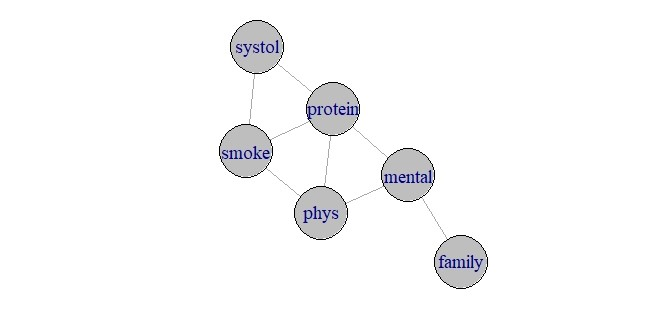
\includegraphics[width=\linewidth]{reinis-aic-forward.jpeg}
	
	Note that, the above chosen model is \textbf{decomposable}. 
	The RIP ordering is as follows;
	\begin{enumerate}
		\item (Systol, Smoke, Protein) as Clique 1.
		\item (Smoke, Protein, Phys) as Clique 2.
		\item (Protein, Phys, Mental) as Clique 3.
		\item (Mental, Family) as Clique 4.
	\end{enumerate}

	The conditional independences are as follows;
	\begin{enumerate}
		\item Systol $\indep$ (Phys, Mental, Family) $\mid$ (Protein, Smoke).
		\item (Systol, Smoke) $\indep$  (Mental, Family) $\mid$ (Protein, Phys).
		\item (Systol, Protein, Smoke, Phys) $\indep$ Family $\mid$ Mental.
	\end{enumerate}
	All other conditional independences follow from taking subset of one or both of the independent sets and increasing the size of conditioning set. Hence, in a sense, all other conditional independences can be derived from the above relations.
	
	The AIC of the above model is 13371.18 and BIC is 13464.99. Next, we perform backward model selection using AIC.
	
	\begin{lstlisting}[style = R-code]
	# backward model selection using AIC starting from saturated model
	fit.backward <- stepwise(dm.sat, criterion = "aic", direction = "backward", type = "unrestricted", k = 2)
	iplot(fit.backward)
	\end{lstlisting}
	
	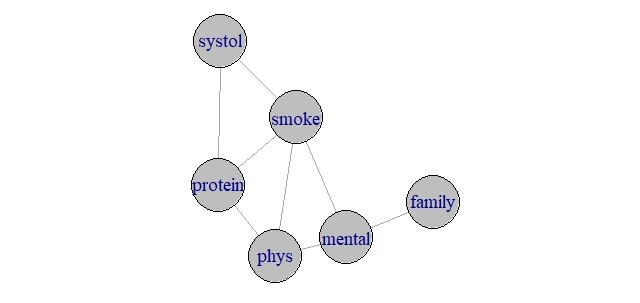
\includegraphics[width=\linewidth]{reinis-aic-backward.jpeg}
	
	Note that, this model is essentially very similar to the one before. It is decomposable. The RIP ordering is as follows;
	\begin{enumerate}
		\item (Systol, Smoke, Protein) as Clique 1.
		\item (Smoke, Protein, Phys) as Clique 2.
		\item (Smoke, Phys, Mental) as Clique 3.
		\item (Mental, Family) as Clique 4.
	\end{enumerate}
	
	The conditional independences are as follows;
	\begin{enumerate}
		\item Systol $\indep$ (Phys, Mental, Family) $\mid$ (Protein, Smoke).
		\item (Systol, Protein) $\indep$  (Mental, Family) $\mid$ (Smoke, Phys).
		\item (Systol, Protein, Smoke, Phys) $\indep$ Family $\mid$ Mental.
	\end{enumerate}
	All other conditional independences follow from taking subset of one or both of the independent sets and increasing the size of conditioning set. Hence, in a sense, all other conditional independences can be derived from the above relations.
	
	
	The AIC of the above model is 13371.63 and BIC is 13465.43, which is pretty close to the selected model before.
	
	To perform BIC based model selection, we essentially use the same code, but with $k = \log n$, where $n$ is the total number of observations. The \textbf{R} function \texttt{stepwise} uses the model selection criteria, $-2\log L + kp$, where $p$ is the number of parameters and $k$ is the penalty parameter passed as an argument in the function.
	
	\begin{lstlisting}[style = R-code]
	# forward model selection using bic
	fit.forward <- stepwise(dm.null, criterion = "aic", direction = "forward", type = "unrestricted", k = log(sum(reinis)))
	iplot(fit.forward)
	\end{lstlisting}
	
	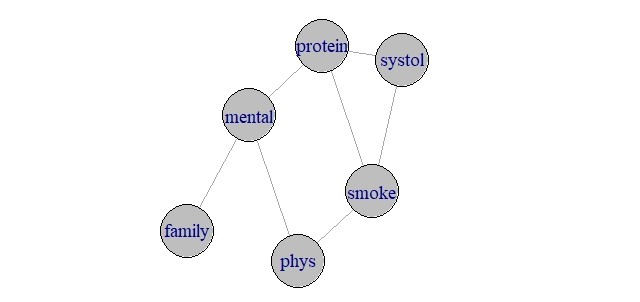
\includegraphics[width=\linewidth]{reinis-bic-forward.jpeg}
	
	The above model is not decomposable, since (Protein, Smoke, Phys, Mental) is a chordless cycle of length 4. The AIC of the selected model is 13372.55 and the BIC is the selected model is 13449.8.
	
	The conditional independences are as follows;
	\begin{enumerate}
		\item Systol $\indep$ (Phys, Mental, Family) $\mid$ (Protein, Smoke).
		\item (Systol, Smoke) $\indep$  (Mental, Family) $\mid$ (Protein, Phys).
		\item (Systol, Protein) $\indep$ Family $\indep$ Phys $\mid$ (Smoke, Mental).
		\item (Systol, Protein, Smoke, Phys) $\indep$ Family $\mid$ Mental.
	\end{enumerate}
	All other conditional independences follow from taking subset of one or both of the independent sets and increasing the size of conditioning set. Hence, in a sense, all other conditional independences can be derived from the above relations. Next, we use backward selection using BIC based criterion.
	
	\begin{lstlisting}[style = R-code]
		# backward model selection
		fit.backward <- stepwise(dm.sat, criterion = "aic", direction = "backward", type = "unrestricted", k = log(sum(reinis)))
		iplot(fit.backward)
	\end{lstlisting}
	
	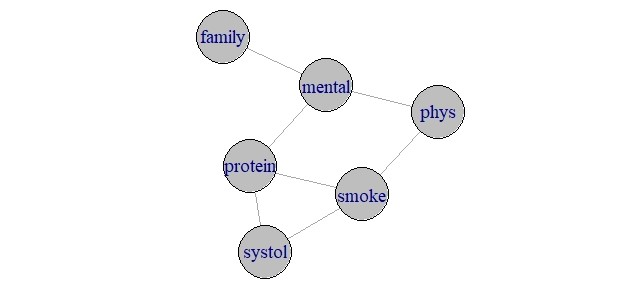
\includegraphics[width=\linewidth]{reinis-bic-backward.jpeg}
	
	The selected model turns out to be same as the one selected by forward selection. Hence, it is not decomposable and the conditional independences are same as before.
	
	In terms of AIC, the first model seems substantially better than the third model, while only marginally better than the second model. On the other hand, in terms of BIC, third model is substantially better than the first and second model. The first model being decomposable, is easy to work with for finding the maximum likelihood estimator.
	
	
	\item[(ii)] Firstly, we load the dataset into \textbf{R} using the following code.
	
	\begin{lstlisting}[style = R-code]
		deathpenalty <- array(c(19, 132, 11, 52, 0, 9, 6, 97), dim = c(2,2,2), dimnames = list("Death.penalty" = c("Yes", "No"), "Defendant.race"= c("White","Black"), "Victim.race" = c("White","Black")))
		ftable(deathpenalty)
	\end{lstlisting}
	
	\begin{lstlisting}[style = R-output]
		                             Victim.race White Black
		Death.penalty Defendant.race                        
		Yes           White                         19     0
					  Black                         11     6
		No            White                        132     9
					  Black                         52    97
	\end{lstlisting}
	We first fit a saturated and an independence model for the data.
	
	\begin{lstlisting}[style = R-code]
		dm.sat <- dmod( ~ . ^ ., as.table(deathpenalty)) # fit saturated model
		dm.null <- dmod( ~ . ^ 1, as.table(deathpenalty))   # fit independence model
	\end{lstlisting}
	
	We now perform AIC based forward and backward model selection.
	
	\begin{lstlisting}[style = R-code]
		# forward model selection using AIC
		fit.forward <- stepwise(dm.null, criterion = "aic", direction = "forward", type = "unrestricted", k = 2)
		iplot(fit.forward)
	\end{lstlisting}
	 
	 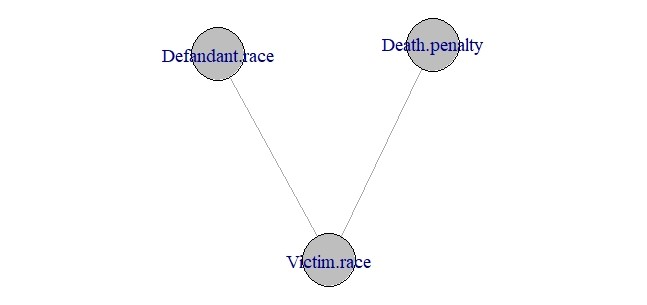
\includegraphics[width=\linewidth]{dp-aic-forward.jpeg}
	 
	 The model is trivially decomposable. The AIC of the model is 971.7625 and BIC of the model is 990.697.
	 
	 The only conditional independence in the model is that; Death Penalty $\indep$ Defendant's Race $\mid$ Victim's Race. Next, we apply the backward selection method. 
	 
	 
	 \begin{lstlisting}[style = R-code]
	 	# backward model selection using AIC
	 	fit.backward <- stepwise(dm.sat, criterion = "aic", direction = "backward", type = "unrestricted", k = 2)
	 	iplot(fit.backward)
	 \end{lstlisting}
	
	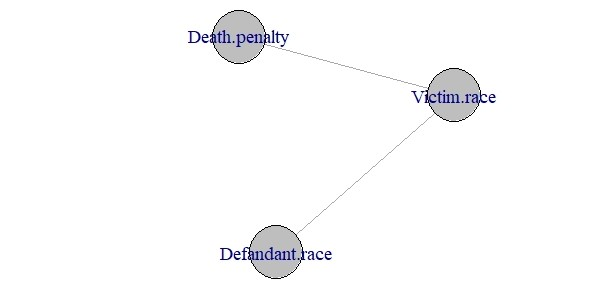
\includegraphics[width=\linewidth]{dp-aic-backward.jpeg}
	
	Note that, the same model is chosen again based on AIC criterion from backward selection.
	
	
	To perform forward and backward model selection based on BIC criterion, we apply the same code again.
	
	\begin{lstlisting}[style = R-code]
		# forward model selection using BIC
		fit.forward <- stepwise(dm.null, criterion = "aic", direction = "forward", type = "unrestricted", k = log(sum(deathpenalty)))
		iplot(fit.forward)
		
		# backward model selection using BIC
		fit.backward <- stepwise(dm.sat, criterion = "aic", direction = "backward", type = "unrestricted", k = log(sum(deathpenalty)))
		iplot(fit.backward)
	\end{lstlisting}
	
	Both the above selected model gives the same model as above.
	
	
	Now, following is the code for Iterative Proportional Scaling (IPS) Algorithm implemented from scratch using \textbf{R}. We use the package \textbf{gRbase} for different utility functions such as slicing and marginalization.
	
	\begin{lstlisting}[style = R-code]
		IPS <- function(form, data, maxiter = 1000, tol = 1e-05) {
		# initialize an array of 1's only
		tempdata <- array(1, dim = dim(data), dimnames = dimnames(data))
		form.vars <- labels(terms(formula(form)))
		
		current_error <- Inf
		current_iter <- 0
		while (current_error > tol & current_iter < maxiter) {
		# store the current table for computing the error later
		current_tab <- tempdata
		
		# for each given margin, perform the updation
		for (var in rev(form.vars))   {
		true_margins <- ar_marg(data, formula(paste0("~", var)))   # compute the true marginals
		current_margins <- ar_marg(tempdata, formula(paste0("~", var)))   # compute the current margins
		
		# expand them to higher dimension as original so that multiplication can be performed
		true_margins <- ar_expand(true_margins, dimnames(data))    
		current_margins <- ar_expand(current_margins, dimnames(data))
		
		tempdata <- (tempdata * true_margins)/current_margins
		}
		
		current_iter <- current_iter+ 1        # increase number of iteration
		current_error <- max(abs(tempdata - current_tab))   # compute the error
		}
		
		return(list("MLE Table" = tempdata, "Iteration" = current_iter))
		}
	\end{lstlisting}
	
	Now, we call the above function to find maximum likelihood estimators under model (a).
	\begin{lstlisting}[style = R-code]
		IPS( ~ Victim.race + Death.penalty + Defendant.race + Victim.race:Death.penalty + 
		Death.penalty:Defendant.race + Victim.race:Defendant.race, deathpenalty)
	\end{lstlisting}
	\begin{lstlisting}[style = R-output]
		$`MLE Table`
		, , Victim.race = White
		
		Defendant.race
		Death.penalty     	White    	Black
		Yes  				18.67436 	11.32564
		No  				132.32564 	51.67436
		
		, , Victim.race = Black
		
		Defendant.race
		Death.penalty     	White     	Black
		Yes 				0.3256423  	5.674358
		No  				8.6743584 	97.325642
		
		$Iteration
		[1] 11
	\end{lstlisting}
	Note that, the maximum likelihood table is extremely close to the true table. The maximum likelihood estimate of $m_{\text{Black, White, No}} = 8.674$, which is pretty close to the true value.
	
	Now, we call the above function again to find maximum likelihood estimators under model (b).
	\begin{lstlisting}[style = R-code]
	IPS( ~ Victim.race + Death.penalty + Defendant.race + Victim.race:Defendant.race + Victim.race:Death.penalty, deathpenalty)
	\end{lstlisting}
	\begin{lstlisting}[style = R-output]
	$`MLE Table`
	, , Victim.race = White
	
	Defendant.race
	Death.penalty     	White     	Black
	Yes  				21.16822  	8.831776
	No  				129.83178 	54.168224
	
	, , Victim.race = Black
	
	Defendant.race
	Death.penalty     	White     	Black
	Yes 				0.4821429  	5.517857
	No  				8.5178571 	97.482143
	
	$Iteration
	[1] 2
	\end{lstlisting}
	The maximum likelihood estimate of $m_{\text{Black, White, No}} = 8.5178$, which is pretty close to the true value of $9$.
	
	Note that, IPS converges in two iterations for the case of model (b). 
	
	Now, to test the hypothesis $H_0: \text{Model (b)}$ vs $H_1: \text{Model (a)}$, we use a likelihood ratio test.
	
	For $H_0$, under model (b), we have the value of log likelihood is $(-480.8812)$ and the corresponding number of free parameters is $5$. While, under $H_1$, model (a), the value of log likelihood turns out to be $(-480.2907)$, which $6$ free parameters. Hence,
	
	$$-2\log\lambda = -2\log\frac{L_{H_0}}{L_{H_0 \cup H_1}} = -2(\log L_{H_0} - \log L_{H_1}) = 1.181$$
	since, $H_0 \cup H_1 = H_1$, as $H_0 \subset H_1$. Note that, the above likelihood ratio statistic asymptotically follows central chi-squared distribution with degrees of freedom $(6-5) = 1$. The observed chi-square statistic assumes a p-value of $0.2771525$, which is greater than the significance level of $\alpha = 0.05$, hence we fail to reject the null hypothesis in favour of the alternative and richer model (a). 
	
	Hence, we can accept Model (b) as an possibly appropriate model for the given data. Also note that, this model is suggested based on AIC or BIC criterion above.
	
	
\end{enumerate}

\end{solution*}
\end{document}



